\documentclass[../../main.tex]{subfiles}
\begin{document}
\subsection{Software Architektur Konzept}
Das Konzept der Software Architekur beinhaltet zwei verschiedene Konzepte.
Einerseits gibt es ein Konzept welches mehrere Programme beinhaltet welche über eine Middleware miteinander kommunizieren. \\
Andererseits ein Konzept welches aus verschiedenen Komponenten besteht die über Interfaces miteinander interagieren. \\

\subsubsection{Software Architektur mit verschiedenen Komponenten}
\begin{figure}[H] %Architektur ohne Middleware
    \centering
    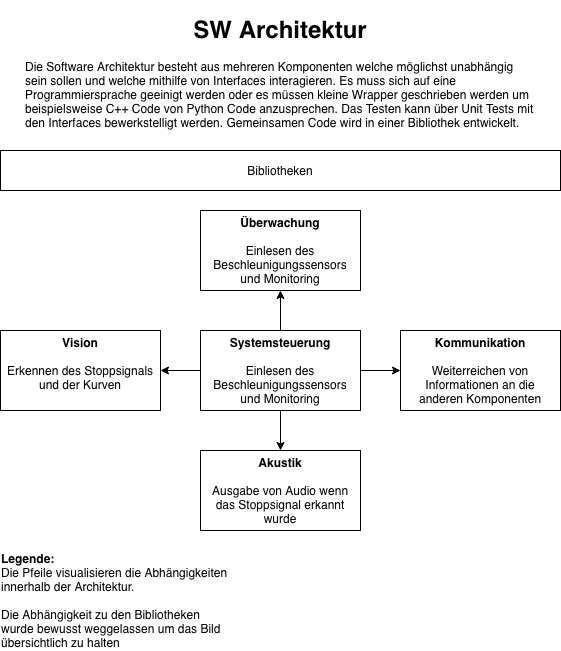
\includegraphics[width=0.6\textwidth]{../../drawings/ArchitekturDiagramm/SW_Architektur.png}
    \caption {Software Architektur Komponenten. Gezeichnet mit https://draw.io}
\end{figure}

\subsubsection{Software Architektur mit Middleware}
\begin{figure}[H] %Architektur ohne Middleware
    \centering
    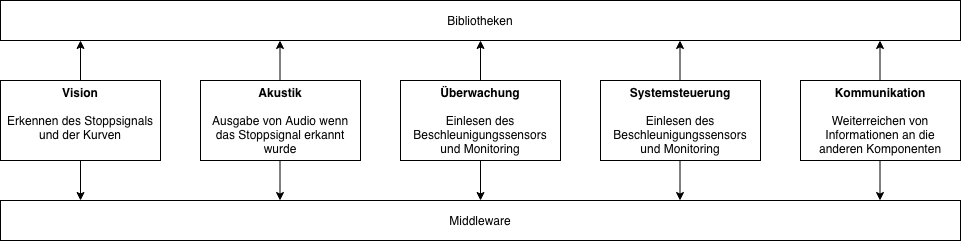
\includegraphics[width=1.0\textwidth]{../../drawings/ArchitekturDiagramm/SW_Architektur_Middleware.png}
    \caption {Software Architektur Middleware. Gezeichnet mit https://draw.io}
\end{figure}

\end{document}